\section{实验}
\label{sec:experiments}
 
我们用了两种方法将我们的方法应用于WMT'14英语到法语机器翻译(MT)任务中。 我们使用它直接翻译输入句子而不参考统计机器翻译(SMT)系统,我们使用它来重新定义SMT基准的n个最佳列表。我们报告这些翻译方法的准确性,
呈现示例翻译,并可视化所得到的句子结果。

\subsection{数据集细节}

我们使用WMT'14英语到法语数据集。我们训练我们的模型在12M句子的一个子集包括348M法语单词和304M英语单词,这是一个来自\cite{wmt14_en_fr}的“选择”过的干净的子集。我们选择这个翻译任务和这个具体训练集子集,是因为分过词的(tokenized)训练和测试集以及来自基准SMT的1000个最佳列表是公共可用的\cite{wmt14_en_fr}。

因为典型的神经语言模型依赖于每个词的向量表示,我们为这两种语言使用固定的词汇。我们用了
源语言里最常见的160,000个单词和目标语言里最常用的8万个单词。每一个
超纲单词都被替换为一个特殊的“UNK”符号。  
 
%% \subsection{Sentence-level Autoencoder}

%% To solve our translation task, the LSTM must store the entire input
%% sentence in its memory, and it is not clear that an LSTM can learn to
%% store the necessary amount of information in its hidden state.  Thus,
%% we start with the easier problem of memorizing an input sentence by
%% reading it into the hidden state and then outputting the same
%% sentence.  If this autoencoding task proves to be too difficult for
%% the LSTM, it would mean that our approach is relatively hopeless.

%% Luckily, we found that the LSTM could easily solve the memorization
%% problem, as it has achieved a perplexity of $1.03$ on the test set.
%% This very low perplexity suggests that at minimum, the LSTM is capable
%% of learning to store a sequence of words of an unknown length in a
%% vector of a fixed dimensionality.


\subsection{解码和重新计算}

我们实验的核心涉及在许多句子对上训练大型深度LSTM。我们通过最大化给定原句子$S$得出正确翻译$T$的概率的对数来训练它,所以训练的目标函数是
$$1/|\mathcal S|\sum_{(T,S)\in\mathcal S}\log p(T|S)$$ 其中 $\mathcal
S$ 是训练集。一旦训练完成,我们根据LSTM找到最有可能的翻译从而生成翻译:
\begin{equation}
\label{eqn:decode}
\hat{T} = \arg\max_T p(T|S)
\end{equation}
我们使用一个简单的从左到右集束搜索(beam search)的解码器来查找最有可能的翻译,这个解码器保持着一个数目为$B$的部分假设(partial hypothesis),其中一个部分假设是一些译文的前缀。在每个时间步长我们用词汇表中每个可能的单词扩展在束(beam)中的每个部分假设。这大大增加了假设(hypothesis)的数量,所以我们根据模型的对数概率舍弃所有除了$B$最可能的假设。一旦``$<$EOS$>$''符号添加到假设中,它就从束中移除,并被添加到完整假设的集合中。虽然这个解码器是近似的,但实施起来很简单。有趣的是,我们的系统即使在束尺寸为1的情况下也表现良好,束尺寸为2时提供了集束搜索的大部分益处(表格
\ref{tab:blue_fr})。

% todo:  insert note on removing very short solutions and solutions
% that consist entirely of the /UNK/ token. 

我们还使用LSTM来分析基准系统生成的1000个最佳列表\cite{wmt14_en_fr}。为了分析n最佳列表,我们使用我们的LSTM计算每个假设的对数概率,并且用他们的分数和LSTM的分数取了平均值。

\subsection{反转源句子}
\label{sec:rev_rev}

虽然LSTM能够解决长期依赖(long term dependencies)的问题,但我们发现,当源语句颠倒(目标语句不反转)时,LSTM学习得更好。通过这样做,LSTM的测试困惑度(perplexity)从5.8下降到4.7,测试其解码翻译的BLEU分数从25.9增加到30.6。



虽然我们没有这种现象的完整解释,但我们认为它是由对数据集引入许多短期依赖(short term dependencies)引起的。通常,当我们将源语句与目标语句连接起来时,源语句中的每个单词远离目标语句中的相应单词。结果是,该问题具有大的``最小时间滞后''\cite{minimal_time_lag}。通过反转源语句中的单词,源语言和目标语言中相应单词之间的平均距离不变。然而,源语言中的前几个词现在非常接近目标语言中的前几个词,所以这个问题的最小时间滞后被大大减少了。因此,反向传播(backpropagation)在源句子和目标句子之间更容易“建立通信”,这又导致整体性能有了实质上的改善。

最初,我们认为,颠倒输入的句子只会导致在目标句子的前面部分中预测的更有信心,而在后面的部分中预测的更不自信。然而,用反向源语句训练的LSTM比直接用源语句训练的LSTM效果好的多(参见
章节 ~\ref{sec:long_sentences}),这表明逆转输入句子导致LSTM具有更好的内存利用率。



%% This result also suggests that hidden optimization issues are still
%% prevalent even in modern-day neural networks.  Prior to training LSTMs
%% on the reversed dataset, we believed that our models were
%% well-optimized, and that little could be gained with better
%% optimization methods.  However, the same architecture is clearly
%% capable of achieving much better results on essentially the same data, which
%% suggests that the worse performance of the ``forward'' LSTMs were entirely
%% due an optimization failure. 

%% \subsection{The Importance of Depth}

%% Deep LSTMs turned out to be important for MT tasks.  In earlier
%% experiments, we found that each additional layer reduced perplexity by
%% 10\%.  As we do not observe such perplexity reductions with deep LSTMs
%% on language modelling, it follows that most of the benefit of deep
%% LSTMs comes from their larger hidden state, which is important for our
%% formulation of MT where the hidden state needs to store the entire
%% input sentence.

\subsection{训练细节}

我们发现LSTM模型是相当容易训练。我们使用具有4层深度的LSTM,每层1000个神经单元和1000
维词嵌入,输入词汇为160,000,输出词汇为80,000。因此深层LSTM使用8000个实数来表示一个句子。我们发现深层LSTM明显优于浅层LSTM,其中每个附加层将困惑度降低近 10\%,可能是由于它们隐藏状态(hidden state)更大。  在每一个输出层,我们使用一个简单的,超过80,000个单词的softmax。
所得到的LSTM具有384M个参数,其中64M是纯
循环连接的(32M用于“编码器”LSTM,32M用于
``解码器''LSTM)。 完整的训练详情如下:
\begin{itemize}
\item 我们用-0.08到0.08的均匀分布初始化了所有的LSTM参数
\item 我们使用没有动量的随机梯度下降,固定学习率为0.7。 在5次迭代(epoch)之后,我们开始每半次迭代就将学习速率减半。我们的模型一共迭代了7.5次。
\item 我们设置批次(batch)的大小为128
\item 虽然LSTM倾向于不遭受梯度消失(vanishing gradient)的问题,但是它们会有梯度爆炸(exploding gradient)。因此,我们通过在梯度的范数超过阈值时对其进行缩放来对梯度的范数实施硬约束\cite{graves13c,razvan}。对于每一个训练批次,我们计算 $s =
  \left\|g\right\|_2$, 其中 $g$ 是 128除以梯度的值。如果 $s > 5$, 我们设
  $g = \frac{5g}{s}$.
\item 不同的句子有不同的长度。大多数句子较
短(例如,长度20-30),但一些句子很长(例如,长度
  $>$ 100),因此,128个随机选择的训练句子的小批(minibatch)处理将具有许多短句和很少的长句子,并且作为结果,小批量中的大量计算被浪费。为了解决这个问题,我们确保在一个小批中的所有句子大致有相同的长度,从而产生一个2倍加速。
\end{itemize}


\subsection{Parallelization}

A C++ implementation of deep LSTM with the configuration from the
previous section on a single GPU processes a speed of approximately
1,700 words per second.  This was too slow for our purposes, so we 
parallelized our model using an 8-GPU machine.  Each layer of the LSTM
was executed on a different GPU and communicated its activations
to the next GPU / layer as soon as they were computed.  Our models
have 4 layers of LSTMs, each of which resides on a separate GPU.  The remaining
4 GPUs were used to parallelize the softmax, so each GPU was
responsible for multiplying by a $1000\times 20000$ matrix.  The
resulting implementation achieved a speed of 6,300 (both English and
French) words per second with a minibatch size of 128. 
Training took about a ten days with this implementation.


\subsection{Experimental Results}

We used the cased BLEU score \cite{bleu} to evaluate the quality of our
translations. We computed our BLEU scores using \texttt{multi-bleu.pl}\footnote{
There several variants of the BLEU score, and each variant is defined  with a perl script. } 
on the \emph{tokenized} predictions and ground truth.
This way of evaluating the BELU score is consistent with \cite{cho14} and \cite{bog14}, and reproduces
the 33.3 score of \cite{wmt14_en_fr}.
However, if we evaluate the best WMT'14 system \cite{durrani-EtAl:2014:W14-33}
(whose predictions can be downloaded from \url{statmt.org\matrix}) in this manner, we get   
37.0, which is greater than the 35.8 reported by \url{statmt.org\matrix}.  

%% According to , 
%% the performance of the best English to French system on the WMT'14 \cite{durrani-EtAl:2014:W14-33}
%% is 35.8.  This score is obtained if we use the \texttt{mteval.pl} script on the \emph{untokenized}
%% test set.  We obtain 37.0 if we download the predictions of the best system from 
%% \url{statmt.org\matrix} and use \texttt{multi-bleu.pl} on the \emph{tokenized}
%% predictions.  This is done to be consistent with \cite{cho14} and \cite{bog14}.
%% All our scores 



%% We verified the correctness of our BLEU score
%% computation by reproducing the BLEU score of LIUM's baseline system using
%% its n-best list. Of particular importance were issues relating to
%% tokenization and normalization of the test sentences.  We made sure to ``unnormalize'' our
%% translations (for example, to replace ``they 're'' with ``they're''),
%% in order to reproducing the baseline's BLEU score with our
%% evaluation tools.

The results are presented in tables \ref{tab:blue_fr} and
\ref{tab:blue_fr_rescore}.  Our best results are obtained with an
ensemble of LSTMs that differ in their random initializations and
in the random order of minibatches.  While the decoded translations of the
LSTM ensemble do not outperform the best WMT'14 system, it is the first time
that a pure neural translation system outperforms a 
phrase-based SMT baseline on a large scale MT task by a sizeable margin,
despite its inability to handle out-of-vocabulary words.  The LSTM
is within 0.5 BLEU points of the best WMT'14 result if it is used to rescore the 1000-best
list of the baseline system.

\begin{table}[t]
\centering
\begin{small}
\begin{tabular}{|c|c|}
\hline
{\bf Method}  & {\bf test BLEU score (ntst14) } \\ \hline
Bahdanau et al. \cite{bog14}  &  28.45 \\ \hline
Baseline System  \cite{wmt14_en_fr} & 33.30 \\ \hline
\hline
Single forward LSTM, beam size 12 & 26.17 \\ \hline                 
Single reversed LSTM, beam size 12 & 30.59 \\ \hline
Ensemble of 5 reversed LSTMs, beam size 1  &  33.00 \\ \hline
Ensemble of 2 reversed LSTMs, beam size 12  &  33.27 \\ \hline
Ensemble of 5 reversed LSTMs, beam size 2  &  34.50 \\ \hline
Ensemble of 5 reversed LSTMs, beam size 12  &  {\bf 34.81} \\ \hline
\end{tabular}
\end{small}
\caption{The performance of the LSTM on WMT'14 English to French test
  set (ntst14).  Note that an ensemble of 5 LSTMs with a beam of size
  2 is cheaper than of a single LSTM with a beam of size 12.  }
\label{tab:blue_fr}
\end{table}

\begin{table}[]
\centering
\begin{small}
\begin{tabular}{|c|c|}
\hline
{\bf Method}  & {\bf test BLEU score (ntst14) } \\ \hline
Baseline System  \cite{wmt14_en_fr} & 33.30 \\ \hline
Cho et al. \cite{cho14}  & 34.54 \\ \hline 
Best WMT'14 result \cite{durrani-EtAl:2014:W14-33} &  {\bf 37.0} \\ \hline
\hline
Rescoring the baseline 1000-best with a single forward LSTM & 35.61 \\ \hline 
Rescoring the baseline 1000-best with a single reversed  LSTM & 35.85 \\ \hline  %wmt_FREN_good_rescore_80k_one_rev_1.merge
%Rescoring the LIUM 1000-best with 5 forward LSTMs  &  36.3 \\ \hline    
Rescoring the baseline 1000-best with an ensemble of 5 reversed LSTMs  &  {\bf 36.5} \\ \hline    %wmt_FREN_good_rescore_80k_all_rev_1.merge 
\hline
Oracle Rescoring of the Baseline 1000-best lists    & $\sim$45 \\ \hline 
\end{tabular}
\end{small}
\caption{Methods that use neural networks together with an SMT system
  on the WMT'14 English to French test set (ntst14).}
\label{tab:blue_fr_rescore}
\end{table}



\subsection{Performance on long sentences}
\label{sec:long_sentences}

We were surprised to discover that the LSTM did well on long
sentences, which is shown quantitatively in figure \ref{fig:oriol}.
Table \ref{tab:examples} presents several examples of long sentences and
their translations. 

\begin{table}[ht!]
\centering
\begin{footnotesize}
\begin{tabular}{|l|l|}
\hline
{\bf  Type} & {\bf Sentence} \\ 
\hline
\hline
{\bf Our model} & Ulrich UNK , membre du conseil d' administration du constructeur automobile Audi , \\
& affirme qu' il s' agit d' une pratique courante depuis des ann\'{e}es pour que les t\'{e}l\'{e}phones \\
& portables  puissent  \^{e}tre collect\'{e}s avant les r\'{e}unions du conseil d' administration afin qu' ils\\
&  ne soient pas  utilis\'{e}s comme appareils d' \'{e}coute \`{a} distance .\\
%%Ulrich UNK , membre du conseil d'administration du constructeur automobile Audi  \\
%%&  , affirme qu'il les r\'{e}unions du s'agit d'une pratique  courante depuis des ann\'{e}es pour      \\
%%& que les t\'{e}l\'{e}phones portables puissent \^{e}tre collect\'{e}s avant conseil d'administration afin     \\
%%& qu'ils ne soient pas utilis\'{e}s comme appareils d'\'{e}coute \`{a} distance . \\
%\hline
%{\bf EN} & UNK Ulrich, a member of the board of automaker Audi says that this is a common  \\
%{\bf LSTM}& practice for years that mobile phones can be collected before the meetings of the board so that  \\
%& they do are not used as remote listening devices. \\
\hline
{\bf  Truth} &  Ulrich Hackenberg , membre du conseil d' administration du constructeur automobile Audi ,   \\
& d\'{e}clare que la collecte des t\'{e}l\'{e}phones portables avant les r\'{e}unions du conseil , afin qu' ils  \\
& ne puissent pas \^{e}tre utilis\'{e}s comme appareils d' \'{e}coute \`{a} distance , est une pratique courante \\ 
& depuis des ann\'{e}es .\\
\hline\hline
%{\bf EN} &  Ulrich Hackenberg, member of the board of automaker Audi said that the  \\
%{\bf Truth} & collection of mobile phones before board meetings, so they can not be used as listening devices  \\
%& remotely, is a common practice for years.\\
{\bf Our model} & 
`` Les t\'{e}l\'{e}phones cellulaires , qui sont vraiment une question , non seulement parce qu' ils \\
& pourraient potentiellement causer des interf\'{e}rences avec les appareils de navigation , mais \\
& nous savons , selon la FCC , qu' ils pourraient interf\'{e}rer avec les tours de t\'{e}l\'{e}phone cellulaire \\
& lorsqu' ils sont dans l' air '' , dit UNK .\\
%%``Les t\'{e}l\'{e}phones cellulaires , qui sont vraiment une question , non seulement parce \\
%%& qu'ils pourraient potentiellement causer des interf\'{e}rences avec les appareils de navigation , \\
%%& mais nous savons , selon la FCC , qu'ils pourraient interf\'{e}rer avec les tours de t\'{e}l\'{e}phone cellulaire \\
%%&  lorsqu'ils sont dans l'air `` , dit UNK .  \\
\hline
{\bf Truth} & 
`` Les t\'{e}l\'{e}phones portables sont v\'{e}ritablement un probl\`{e}me , non seulement parce qu' ils \\
& pourraient \'{e}ventuellement cr\'{e}er des interf\'{e}rences avec les instruments de navigation , mais \\
& parce que nous savons , d' apr\`{e}s la FCC , qu' ils pourraient perturber les antennes-relais de \\
& t\'{e}l\'{e}phonie mobile s' ils sont utilis\'{e}s \`{a} bord '' , a d\'{e}clar\'{e} Rosenker .\\
%%`` Les t\'{e}l\'{e}phones portables sont v\'{e}ritablement un probl\'{e}me , non seulement parce qu'ils \\
%%& pourraient \'{e}ventuellement cr\'{e}er des interf\'{e}rences avec les instruments de navigation , mais parce \\
%%& que nous savons , d'apr\`{e}s la FCC , qu'ils pourraient perturber les antennes-relais de \\
%%& t\'{e}l\'{e}phonie mobile s'ils sont utilis\'{e}s \`{a} bord '' , a d\'{e}clar\'{e} Rosenker . \\
\hline\hline
{\bf Our model} & 
Avec la cr\'{e}mation , il y a un `` sentiment de violence contre le corps d' un \^{e}tre cher '' , \\
& qui sera `` r\'{e}duit \`{a} une pile de cendres '' en tr\`{e}s peu de temps au lieu d' un processus de \\
& d\'{e}composition ``  qui accompagnera les \'{e}tapes du deuil '' .\\
%%Avec la cr\'{e}mation , il y a un `` sentiment de violence contre le corps d'un \^{e}tre cher `` , \\ 
%%& qui sera `` r\'{e}duit \`{a} une pile de cendres `` en tr\`{e}s peu de temps au lieu d'un processus de d\'{e}composition \\
%%&  `` qui accompagnera les \'{e}tapes du deuil `` . \\  
\hline
{\bf Truth} & 
Il y a , avec la cr\'{e}mation , `` une violence faite au corps aim\'{e} '' , \\
& qui va \^{e}tre `` r\'{e}duit \`{a} un tas de cendres '' en tr\`{e}s peu de temps , et non apr\`{e}s un processus de \\
&d\'{e}composition , qui `` accompagnerait les phases du deuil '' .\\
%%Il y a , avec la cr\'{e}mation , `` une violence faite au corps aim\'{e} `` , qui va \^{e}tre `` r\'{e}duit \\
%%&  \`{a} un tas de cendres `` en tr\`{e}s peu de temps , et non apr\`{e}s un processus de d\'{e}composition , qui `` \\
%%&accompagnerait les phases du deuil `` .\\
\hline
\end{tabular}
\end{footnotesize}
\caption{A few examples of long translations produced by the LSTM
  alongside the ground truth translations.  The reader can verify that
  the translations are sensible using Google translate.  }
\label{tab:examples}
\end{table}



%% \begin{table}[ht!]
%% \centering
%% \begin{footnotesize}
%% \begin{tabular}{|l|l|}
%% \hline
%% {\bf  Type} & {\bf Sentence} \\ 
%% \hline
%% {\bf LSTM} & Ulrich UNK , membre du conseil d'administration du constructeur automobile Audi  \\
%% &  , affirme qu'il les réunions du s'agit d'une pratique  courante depuis des années pour      \\
%% & que les téléphones portables puissent être collectés avant conseil d'administration afin   	  \\
%% & qu'ils ne soient pas utilisés comme appareils d'écoute à distance . \\
%% %\hline
%% %{\bf EN} & UNK Ulrich, a member of the board of automaker Audi says that this is a common  \\
%% %{\bf LSTM}& practice for years that mobile phones can be collected before the meetings of the board so that  \\
%% %& they do are not used as remote listening devices. \\
%% \hline
%% {\bf  Truth} &  Ulrich Hackenberg , membre du conseil d'administration du constructeur    \\
%% & automobile Audi , déclare que la des téléphones portables avant les réunions du conseil , afin qu'ils  \\
%% & ne puissent pas être utilisés comme appareils collecte d'écoute à distance ,  \\
%% &  est une pratique courante depuis des années . \\
%% \hline\hline
%% %{\bf EN} &  Ulrich Hackenberg, member of the board of automaker Audi said that the  \\
%% %{\bf Truth} & collection of mobile phones before board meetings, so they can not be used as listening devices  \\
%% %& remotely, is a common practice for years.\\
%% {\bf LSTM} & ``Les téléphones cellulaires , qui sont vraiment une question , non seulement parce \\
%% & qu'ils pourraient potentiellement causer des interférences avec les appareils de navigation , \\
%% & mais nous savons , selon la FCC , qu'ils pourraient interférer avec les tours de téléphone cellulaire \\
%% &  lorsqu'ils sont dans l'air `` , dit UNK .  \\
%% \hline
%% {\bf Truth} & `` Les téléphones portables sont véritablement un problème , non seulement parce qu'ils \\
%% & pourraient éventuellement créer des interférences avec les instruments de navigation , mais parce \\
%% & que nous savons , d'après la FCC , qu'ils pourraient perturber les antennes-relais de \\
%% & téléphonie mobile s'ils sont utilisés à bord '' , a déclaré Rosenker . \\
%% \hline\hline
%% {\bf LSTM} & Avec la crémation , il y a un `` sentiment de violence contre le corps d'un être cher `` , \\ 
%% & qui sera `` réduit à une pile de cendres `` en très peu de temps au lieu d'un processus de décomposition \\
%% &  `` qui accompagnera les étapes du deuil `` . \\  
%% \hline
%% {\bf Truth} & Il y a , avec la crémation , `` une violence faite au corps aimé `` , qui va être `` réduit \\
%% &  à un tas de cendres `` en très peu de temps , et non après un processus de décomposition , qui `` \\
%% &accompagnerait les phases du deuil `` .\\
%% \hline
%% \end{tabular}
%% \end{footnotesize}
%% \caption{The table shows a few examples of long translations produced
%%   by the LSTM together with the ground truth translations.  The reader
%%   can verify using Google translate that the LSTM's translations are  
%%   basically correct.
%%  }
%% \label{tab:examples}
%% \end{table}


\subsection{Model Analysis}

\begin{figure}[h!]
\centering
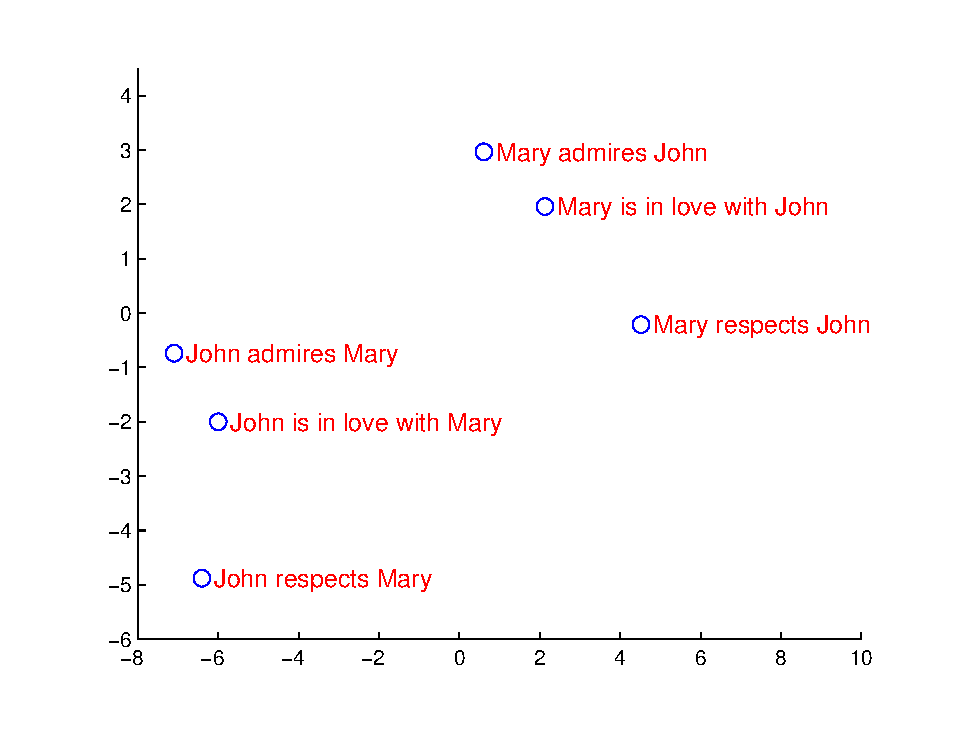
\includegraphics[width=0.46\textwidth]{figure2} ~~
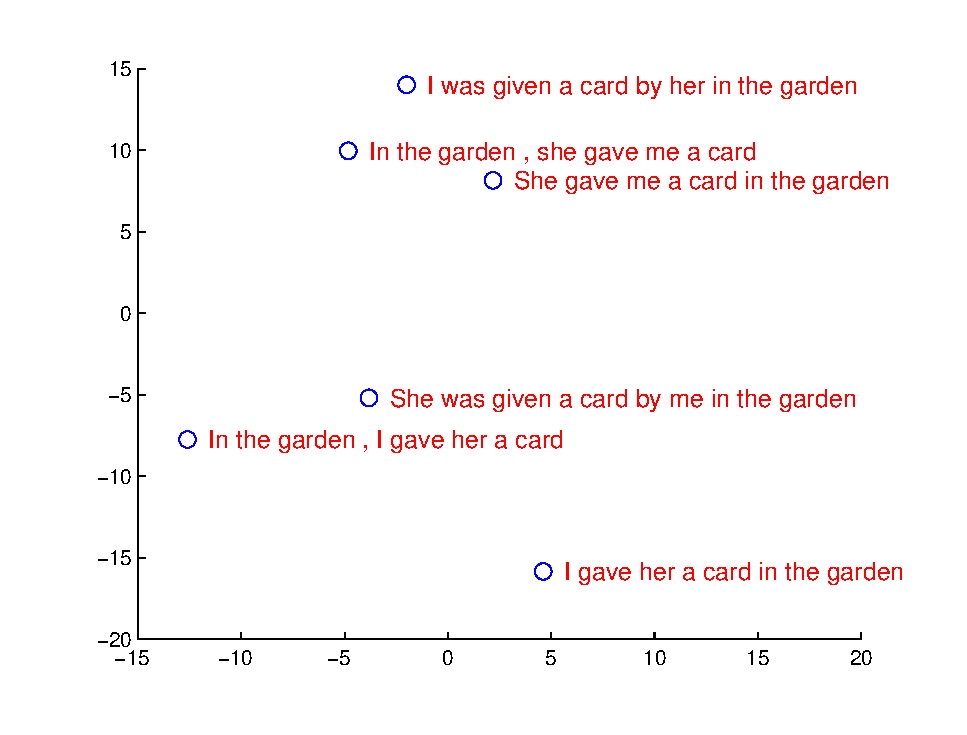
\includegraphics[width=0.46\textwidth]{figure3} 
\caption{\small The figure shows a 2-dimensional PCA projection of the
  LSTM hidden states that are obtained after processing the phrases in
  the figures.  The phrases are clustered by meaning, which in these
  examples is primarily a function of word order, which would be
  difficult to capture with a bag-of-words model. Notice that both
  clusters have similar internal structure.}
\label{fig:embedding}
\end{figure}

%good1} }
\begin{figure}[h!]
\centerline{
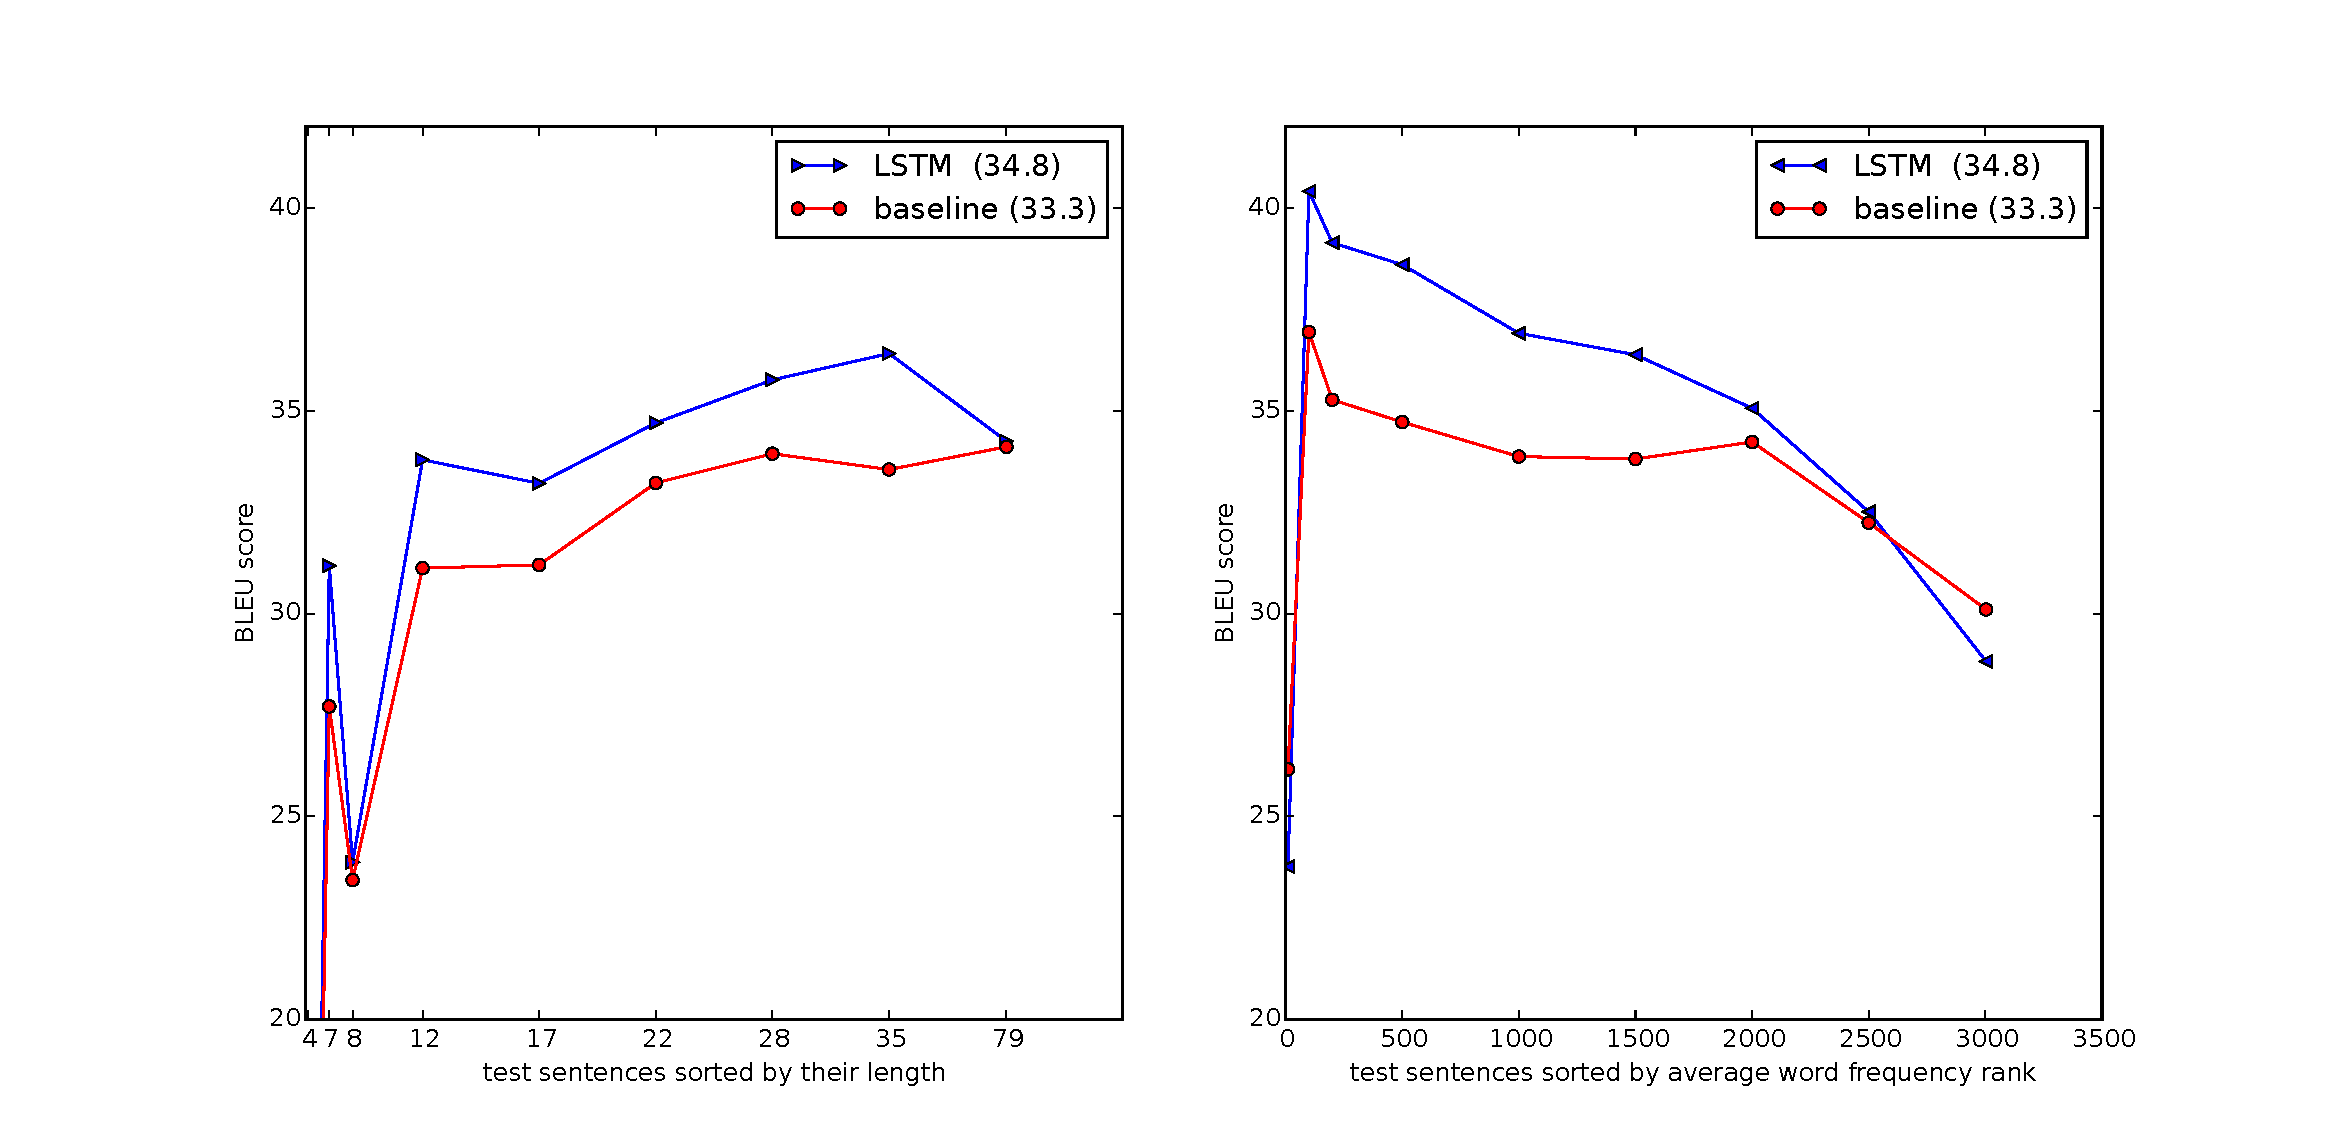
\includegraphics[width=1.\textwidth]{good2.eps} }  
\caption{\small The left plot shows the performance of our system as a
  function of sentence length, where the x-axis corresponds to the
  test sentences sorted by their length and is marked by the actual
  sequence lengths.  There is no degradation on sentences with less
  than 35 words, there is only a minor degradation on the longest
  sentences.  The right plot shows the LSTM's performance on sentences
  with progressively more rare words, where the x-axis corresponds to
  the test sentences sorted by their ``average word frequency rank''.
}
\label{fig:oriol}
\end{figure}

%% In our experiments, we trained LSTMs with only 4 layers, but deeper
%% LSTMs would achieve even better translation performance, every
%% additional LSTM layer reduced the perplexity by almost 10\%.  It is
%% easy to see why it should be so: the deeper LSTMs have much more
%% hidden state, so they have an easier time storing the input sequence.

One of the attractive features of our model is its ability to turn a
sequence of words into a vector of fixed dimensionality.
Figure~\ref{fig:embedding} visualizes some of the learned
representations.  The figure clearly shows that the representations
are sensitive to the order of words, while being fairly insensitive to
the replacement of an active voice with a passive voice.  The
two-dimensional projections are obtained using PCA.






